\chapter{Entrepreneurial Judgment: Mindset, Scale, and Learned Risk}

This interview proceeds by a sequence of pointed questions, but beneath the interview format there is a fairly coherent mathematical spine. Lavon Perrin keeps returning to the same small set of operative variables: peer environment, mindset, usable hours, target size, replication, risk, and management capacity. None of these is developed as a theorem. Still, the lecture does more than trade in slogans. Again and again, it turns a broad entrepreneurial claim into an explicit mechanism, and that is what we preserve here.

\section{The Opening Claim: We Drift Toward Our Environment}

Before the host introduces the series, the lecture opens with a proverb. If we spend time with nine broke friends, we become the tenth. If we spend time with nine people driving Ferraris, our odds improve. This is not presented as social science. It is presented as a compressed operating rule. The lecture begins by insisting that environment is already doing arithmetic on us, whether or not we notice it.

A cautious transcription of that opening heuristic is
\begin{align}
n &= 9, \qquad \text{peers} = \text{broke}
\quad \Longrightarrow \quad
\text{self} \to \text{10th broke peer},\\
n &= 9, \qquad \text{peers} = \text{ambitious}
\quad \Longrightarrow \quad
P(\text{upward move}) \uparrow .
\end{align}

\begin{remark}
These arrows are heuristic rather than literal. Perrin is not claiming a deterministic law; he is claiming that repeated exposure changes aspiration, conduct, and therefore outcome.
\end{remark}

Only after this teaser does the host identify the setting, announce the ``10 Questions with Millionaires'' format, and ask the first formal question: what is the biggest thing that separates people in business? The lecture is already structured. First comes the memorable image; only then comes the explanatory problem.

\section{Mindset as the First Operative Variable}

Perrin's first direct answer is that the separator is mindset. He even says that he could almost stop there. But of course he does not stop there, and that is important. The lecture does not leave ``mindset'' as a motivational word. It immediately tries to tell us what the word does.

\begin{definition}
In this lecture, mindset is the interpretive structure that sits between a situation and the action taken in response to it. It determines whether the situation is read as possibility, obstruction, or excuse.
\end{definition}

A useful reconstruction is
\begin{equation}
\text{Situation} + \text{Mindset} \to \text{Interpretation} \to \text{Action}.
\end{equation}

This is why the answer widens so quickly from business performance to the news, negativity, and self-accountability. If the interpretive mechanism is damaged, then even neutral circumstances are processed as negative ones. He is not recommending a vague optimism. He is recommending control over inputs and honesty about outputs. The news example matters because it says that mindset is trained, and trained by repeated exposure.

That is also why the next move in the lecture is so sharp. Perrin does not merely say that attitude matters. He asks why one is not where one wants to be, and then answers by directing the listener back toward the mirror. The point is severe: external conditions may be real, but they cannot be allowed to carry the full explanatory burden.

\subsection{Question \& Answer}

\paragraph{Question.} If mindset is the decisive tool, where do we first see it changing outcomes rather than merely changing feelings?

\paragraph{Answer.} We see it at the moment where self-examination turns into a concrete use of time. Perrin moves from the mirror to the side hustle. That is a crucial transition in the lecture. It prevents mindset from remaining psychological vapor. The right mindset is the one that discovers a convertable resource and acts on it.

His example is built on time-zone arithmetic. Some of his people, he says, live on the East Coast but buy a license on the West Coast. That buys them three more working hours each day. If local calling would stop at \(8{:}00\) p.m., then a West Coast market extends the reachable window to \(11{:}00\) p.m.:
\begin{align}
t_{\text{close,East}} &= 20{:}00,\\
t_{\text{close,West}} &= 23{:}00,\\
\Delta t &= t_{\text{close,West}} - t_{\text{close,East}} = 3\ \text{hours}.
\end{align}

This is one of the lecture's clearest pieces of arithmetic. We are meant to see the mechanism, not merely applaud the sentiment. The example unfolds step by step:
\begin{enumerate}
\item Work the primary job during the day.
\item Have dinner and attend family obligations.
\item Return home at \(20{:}00\).
\item Use the West Coast time difference to work until \(23{:}00\).
\item Repeat until the secondary stream is large enough to replace the first job.
\end{enumerate}

The schedule can be summarized as a narrow vertical flow:

\begin{figure}[h]
\centering
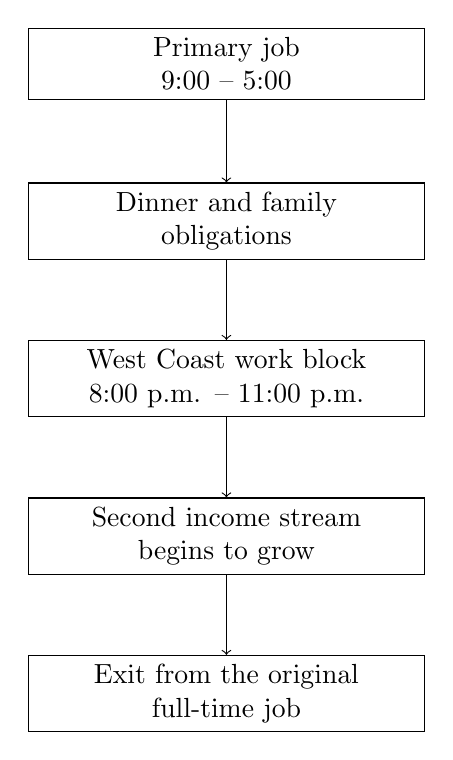
\begin{tikzpicture}
\node[draw, rectangle, text width=4.8cm, align=center] (a) at (0,0) {Primary job\\\(9{:}00\) -- \(5{:}00\)};
\node[draw, rectangle, text width=4.8cm, align=center] (b) at (0,-2.0) {Dinner and family\\obligations};
\node[draw, rectangle, text width=4.8cm, align=center] (c) at (0,-4.0) {West Coast work block\\\(8{:}00\) p.m. -- \(11{:}00\) p.m.};
\node[draw, rectangle, text width=4.8cm, align=center] (d) at (0,-6.0) {Second income stream\\begins to grow};
\node[draw, rectangle, text width=4.8cm, align=center] (e) at (0,-8.0) {Exit from the original\\full-time job};
\draw[->] (a) -- (b);
\draw[->] (b) -- (c);
\draw[->] (c) -- (d);
\draw[->] (d) -- (e);
\end{tikzpicture}
\end{figure}

We should not overread this as a universal business model. Perrin's claim is narrower and stronger. Once mindset ceases to be excuse, time becomes visible again.

\section{From Corporate Misfit to the Entrepreneurial Turn}

The interviewer next asks about the turning point. This comes exactly where it should. After a general claim about mindset and action, the lecture needs a biographical case. Perrin's answer is notable because it resists drama. He does not present entrepreneurship as a sudden revelation. He says, more cautiously, that it just kind of happened.

That caution matters. The lecture is not building a myth of destiny. It is building an account of mismatch, apprenticeship, and eventual independence. Corporate America did not feel like a natural fit. He had too many questions, he bucked the system, yet he was a strong salesperson, was well liked, and could lead people. The tension is productive. The very traits that made him difficult to place inside a corporate setting later became useful in building his own venture.

A compact reconstruction of that logic is
\begin{equation}
\text{Corporate work} \to
\bigl(\text{sales skill} + \text{leadership} + \text{business knowledge}\bigr)
\to \text{independent action}.
\end{equation}

The lecture then sharpens the turning point with a family constraint. Perrin says that in the car business he did not want the personal cost that often came with that world, and he wanted to be able to see his children. The entrepreneurial turn is therefore not explained by ambition alone. It is shaped by the problem of how to work and how to live.

This is also where one of the lecture's quiet strengths appears. Previous employment is not dismissed. It is mined. The tools learned elsewhere are taken and then put into action for oneself. That is the exact phrase the lecture keeps circling around.

\section{Scaling: Targets, Replication, and Chosen Environment}

Once the path into entrepreneurship has been established, the lecture moves to scale. Here Perrin introduces a simple but forceful asymmetry. Many people, he says, want to make \(\$100{,}000\) a year. But that may be part of the problem, because the goal itself is too low. If one were instead to plan for \(\$500{,}000\) and miss, one might still land near \(\$100{,}000\).

We should preserve both the numbers and the caution:
\begin{align}
G_{\text{ordinary}} &= \$100{,}000,\\
G_{\text{stretch}} &= \$500{,}000,\\
Y_{\text{miss stretch}} &\approx \$100{,}000.
\end{align}

\begin{remark}
This is not a statistical model of outcomes. It is a motivational comparison. The point is that a larger target reshapes planning and effort, and therefore changes what a ``miss'' can still produce.
\end{remark}

\subsection{Question \& Answer}

\paragraph{Question.} What actually scales a business?

\paragraph{Answer.} Perrin answers in a sequence: choose a larger target, create a plan, test whether present work is worth reproducing, hold oneself accountable, and then place oneself in a stronger environment. The lecture does not formalize this sequence, but it is clear enough to be written down.

Its most operational piece is the ``10 of me'' test.

\begin{definition}
The ``10 of me'' test asks whether a client, company, or system would be better off if the present standard of performance were multiplied by ten. If the answer is yes, then the work is not merely energetic. It is reproducible.
\end{definition}

A compact reconstruction is
\begin{equation}
\text{Scale-ready}
\iff
\text{Value}(10\times \text{me}) > \text{Value}(1\times \text{me}).
\end{equation}

If ten copies of the present standard would improve the organization, then one is on the right track. If not, scale only multiplies disorder. That is why the lecture joins scale to accountability. Perrin says, in effect: why are you not successful? Up to a point, that answer is about you. We should read that as his provocation, not as a universal theorem about society. But it is central to his sequence.

The section then folds the opening proverb back into the argument. Environment returns, now with fuller force. The Ferrari line is not only about status. It is about normality. If we place ourselves among people who normalize a higher standard of action, then our own conduct is dragged upward.

So we may summarize the final move in the section as
\begin{equation}
\text{better peer set} \to P(\text{better conduct and better outcome}) \uparrow .
\end{equation}

Perrin's move downtown is offered as the concrete instance: he wanted to be around people already living, building, and operating at the level he was aiming toward. He closes the point with another strong maxim: there is no practice life. The chapter should keep that sentence in view, because it is the moral pressure behind the whole scaling discussion.

\section{Risk, Sales, and the Work of Self-Development}

After scale comes the next natural question: what is the price of progress? Perrin's answer is crisp. There is no success without risk. That phrase is not decorative. It is the hinge between aspiration and exposure. If one wants unusual outcomes, one must tolerate uncertainty.

Still, the lecture is careful not to glorify impulsiveness. The risk is to be calculated, joined to self-belief, and joined to education. The functional rule is
\begin{equation}
\text{Action} + \text{Calculated Risk}
\to
\text{Outcome}
\to
\text{Learning}
\to
\text{Better Next Action}.
\end{equation}

This is not the language of probability theory, and we should not pretend that it is. But it is a genuine update rule. One acts, one observes, and one carries the result forward rather than collapsing into either bravado or fear.

\subsection{Question \& Answer}

\paragraph{Question.} What is the secret to sales?

\paragraph{Answer.} The lecture gives a surprising answer: personal development. Perrin does not begin with persuasion tactics. He begins with reading, study, and the work of understanding one's own motives and ambitions. That answer belongs exactly here. Risk has just been defined as something that must be taken intelligently, and now the lecture tells us where intelligence in practice is supposed to come from.

The transcript supplies one concrete measure of this shift:
\begin{equation}
B_{\text{last year}} \approx 15,
\qquad
B_{\text{year before}} \ll B_{\text{last year}}.
\end{equation}

The point is not that fifteen is sacred. The point is that self-development ceased to be an aspiration and became a repeated practice.

The books named in the lecture are:
\begin{itemize}
\item Napoleon Hill's \textit{Think and Grow Rich},
\item \textit{Rich Dad Poor Dad},
\item \textit{Go for No}.
\end{itemize}

The sequencing is essential. First Perrin claims that sales is downstream of personal development. Then he names the books. Then he explains what the books did: they helped him validate why his thoughts were where they were and why his ambitions were focused where they were. In other words, the books matter because they helped change the operator. They did not simply supply slogans.

\section{Owning a Business: Mistakes, Leverage, and Managed Money}

The late lecture turns from aspiration to operation. The host asks about the biggest challenge in owning a business, then about the worst financial decision, then about work-life balance, and finally about money and happiness. The order matters. We are moving from growth to discipline.

Perrin says that one of the biggest challenges is learning how to be a business owner at all. That means consistency, budgeting, growth decisions, and acceptance of the fact that every business has ups and downs. The tone here becomes more sober. Earlier we treated time as a personal block reclaimed from the evening; now we treat entrepreneurship as a repeated exercise in managing fluctuation.

\subsection{Question \& Answer}

\paragraph{Question.} How does an owner learn without being destroyed by mistakes?

\paragraph{Answer.} By refusing two equal and opposite errors: refusing to read every bad outcome as final defeat, and refusing to overanalyze until motion stops. Perrin gives the lecture's cleanest formulation when he says that in business, as in sport, one does not necessarily lose; one learns.

We may write the opposition as
\begin{align}
\text{mistake} &\to \text{lesson},\\
\text{overanalysis} &\to \text{no motion}.
\end{align}

The phrase ``paralysis by analysis'' appears here for a reason. The lecture has already argued that action matters. Now it argues that some forms of thought are actually anti-action. So the owner must learn to distinguish reflection from immobilization.

The BMW anecdote belongs in this operational register. The transcript is rough in spots, but its lesson is still visible. A desired purchase was not condemned in itself. The problem was that it was not handled with enough regard for maintenance and continuing cost. The lecture's meaning is therefore narrower than ``never buy.'' It is
\begin{equation}
\text{purchase without upkeep plan} \to \text{avoidable financial pain}.
\end{equation}

That same structure carries into the discussion of work-life balance. Perrin does not answer with sentiment. He answers with leverage. He points, almost impatiently, to the fact that the person running Amazon has no extra hours in the day. The day itself is fixed:
\begin{equation}
T_{\text{day,Amazon head}} = T_{\text{day,ours}} = 24\ \text{hours}.
\end{equation}

So if outcomes differ radically, the difference must come from structure, delegation, and the intelligent use of time:
\begin{equation}
\text{Output}
=
\text{own effort}
+
\text{leveraged effort of others}.
\end{equation}

This is a late return to a very early theme. At the beginning of the lecture, mindset uncovered usable time in the evening. At the end of the lecture, judgment uncovers usable time inside organization itself.

The last question asks whether money buys happiness. Perrin gives a restrained answer. Money may buy freedom if it is handled properly, but it does not automatically buy happiness. The operative variable is not merely amount. It is management capacity:
\begin{align}
\neg \text{Manage}(\$1{,}000)
&\Longrightarrow
\neg \text{Manage}(\$1{,}000{,}000),\\
\text{Money} + \text{Judgment}
&\to
\text{Freedom},\\
\text{Money}
&\neq
\text{Happiness}.
\end{align}

That is a fitting final turn. The lecture began by saying that environment shapes us. It ends by saying that wealth does not rescue us from poor judgment. It enlarges whatever judgment is already there.

\section{Summary}

Perrin's interview is organized around a single practical question: how do we put ourselves under better rules of interpretation and action? The answers come in a distinct order. First comes peer environment. Then mindset. Then the arithmetic of reclaimed hours. Then the entrepreneurial turn, where previous employment is treated as apprenticeship rather than waste. Then scale, where targets must be large enough, plans concrete enough, and standards reproducible enough to justify growth. Then risk, which must be calculated and converted into learning. Then sales, where personal development is placed beneath technique. Finally come mistakes, leverage, and money management, where the lecture descends from aspiration into operation.

The mathematics is intentionally light, but it is not incidental. Three extra hours matter. A higher target matters. A ``10 of me'' test matters. The ability to manage \(\$1{,}000\) before claiming readiness for \(\$1{,}000{,}000\) matters. In each case the lecture does the same thing: it takes a broad entrepreneurial claim and gives it a mechanism. That is why the opening proverb holds the chapter together. We drift toward the rules, people, and structures around us unless we deliberately choose better ones.